% =============================================================================
%  虚拟结肠镜的数学 · 旗舰讲义（v2，由 English 旗舰经 Phase-6 翻译关得到）
%  把结肠摊平：从「为什么做不到」到一个能手算的方法
%  模式：被动学习讲义 · 主题：teal · 一个驱动问题，深度优先。
%  翻译遵循 zh-technical-style：译意不译词；数学/\TL* 宏/TikZ 坐标与英文版字节一致，只改自然语言串。
%  图：仅用开放授权（CC0），注明出处；不使用任何受版权保护的论文插图。
% =============================================================================
\documentclass[aspectratio=169,10pt]{beamer}
\usepackage[teal]{template-lib/template-lib}
\uselayout{text}
\uselayout{eq}
\uselayout{twocol}

\usetikzlibrary{arrows.meta,calc,positioning,patterns,decorations.pathmorphing,%
  decorations.markings,shapes.geometric,backgrounds}

\newcommand{\R}{\mathbb{R}}
\newcommand{\grad}{\nabla}
\newcommand{\Lap}{\Delta}
\newcommand{\half}{\tfrac{1}{2}}
\newcommand{\inner}[2]{\langle #1,#2\rangle}
\newcommand{\nm}[1]{\lVert #1\rVert}
\newcommand{\xb}{\mathbf{x}}
\newcommand{\Lmat}{\mathbf{L}}
\newcommand{\dd}{\mathrm{d}}

% 本地化「要点」
\renewcommand{\TLtakeaway}[1]{%
  \vspace{0.35em}%
  \begin{tikzpicture}
    \node[fill=TLaccentLight, rounded corners=3pt, inner sep=8pt,
          text width=\linewidth-16pt, align=justify] {%
      \small\textcolor{TLaccent}{\textbf{要点。}} #1%
    };
  \end{tikzpicture}%
  \vspace{0.15em}%
}

\TLsetfoot{把结肠摊平 \textperiodcentered{} 从「为什么做不到」到一个能手算的方法}

\begin{document}

% =============================================================================
\TLtitlecenter
  {把结肠摊平}
  {从「为什么做不到」到一个能手算的方法}
  {虚拟结肠镜的数学 \textperiodcentered{} 旗舰讲义（第一讲）}
  {自学讲义 · 重在重建，而非记忆}

% =============================================================================
\begin{frame}{如何读这份讲义}
  一个问题贯穿全篇：
  \begin{center}
    \emph{我们能不能把弯曲的结肠摊平，让医生一眼看尽每一处肠壁——\\
    又不歪曲息肉的形状？做不到完美的话，能做到多近，又该怎么做？}
  \end{center}
  自学讲义的约定：
  \begin{itemize}
    \item \textbf{每个概念都由一个你已经有的问题引出}——用不到就不提。
    \item \textbf{凡是要紧的结论都当场算出来}，你能用铅笔自己重推。
    \item 我们把\textbf{一个}方法从头做到尾；更深的方法留到末尾，作为后续讲义。
    \item 预备知识：微积分与线性代数。\emph{不需要}微分几何，\emph{不需要}复分析。
  \end{itemize}
  \TLtakeaway{目标：学完能\emph{手动}把一小块网格摊平，并说清它保住了什么、付出了什么、以及为什么这代价无法避免。}
\end{frame}

% =============================================================================
\begin{frame}{五个问题（一页看完整份讲义）}
  \begin{enumerate}
    \item[\textbf{Q1}] 我把结肠剪开、压平——\textbf{哪里出了问题？} \hfill （\emph{度量}）
    \item[\textbf{Q2}] 度量到底什么时候能被抹平？ \hfill （\emph{曲率}；为什么做不到）
    \item[\textbf{Q3}] 既然必须变形，最该保住的是什么？ \hfill （\emph{共形}：保住角度）
    \item[\textbf{Q4}] 在真实的（网格）结肠上到底怎么算？ \hfill （\emph{cotangent Laplacian}）
    \item[\textbf{Q5}] 做出来了吗？代价是多少？ \hfill （量一量；把环闭合）
  \end{enumerate}
  \TLtakeaway{每个问题都逼出下一个概念。Q2 是一个干净的「不行」；Q3--Q5 构造并审计那个退而求其次的方案。}
\end{frame}

% =============================================================================
\TLsection{Q1 · 我把它剪开、压平——哪里出了问题？}

% --- 1.1 the failed experiment ----------------------------------------------
\begin{frame}{一个失败的实验}
  \begin{columns}[T]
    \begin{column}{0.55\textwidth}
      先试最直接的办法。把结肠（一根管子）沿一条线剪开，按到桌面上压平。
      \begin{itemize}
        \item 在肠壁上画一个小三角形，量出它三条边\emph{在曲面上}的长度。
        \item 压平后再量同样这三条边，长度\textbf{变了}——有的被拉长，有的被压短。
      \end{itemize}
      于是有了组织全篇的问题：\emph{如果摊平是「诚实」的，本应保住的是哪个量？}不论它是什么，我们都得先有一把\emph{用曲面自己来量长度}的尺子。
    \end{column}
    \begin{column}{0.45\textwidth}
      \centering
      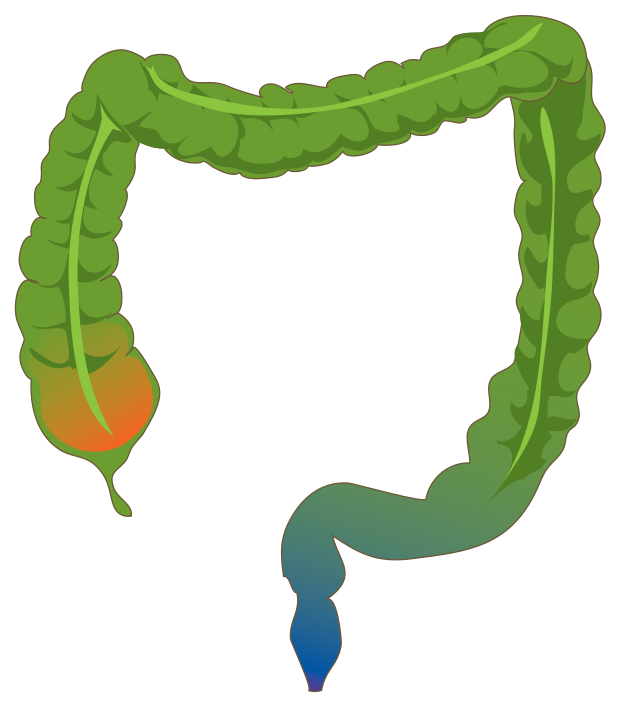
\includegraphics[height=3.5cm]{assets/colon-en/colon_anatomy.png}\\[2pt]
      {\scriptsize 结肠：我们剪开、压平的那根管子。\\
       图：Mikael Häggström，\href{https://commons.wikimedia.org/wiki/File:Colon_(anatomy).svg}{Wikimedia Commons}，公有领域。}
    \end{column}
  \end{columns}
  \TLtakeaway{「无畸变地摊平」必须意味着：\emph{保住曲面自己量出的长度}。所以第一步是造出那把尺子。}
\end{frame}

% --- 1.2 surfaces 101 -------------------------------------------------------
\begin{frame}{曲面是一张映射，它的切向量来量长度}
  把曲面写成从平直参数区到空间的一张映射：
  \[
    \xb(u,v)\in\R^3,\qquad (u,v)\in\Omega\subset\R^2 .
  \]
  \begin{columns}[T]
    \begin{column}{0.6\textwidth}
      \begin{itemize}
        \item \textbf{切向量}就是偏导 $\xb_u=\partial\xb/\partial u$、$\xb_v=\partial\xb/\partial v$。
        \item 参数走一小步 $(\dd u,\dd v)$，你在三维里就挪动了
          \[ \dd\xb=\xb_u\,\dd u+\xb_v\,\dd v , \]
          这一步的真实长度是 $\nm{\dd\xb}$。
        \item 所以它由 $\xb_u,\xb_v$ 和步长算出，全在 $(u,v)$ 里。
      \end{itemize}
      要在曲面上量的一切，都藏在 $\xb_u,\xb_v$ 的三个点积里。
    \end{column}
    \begin{column}{0.4\textwidth}
      \centering
      \begin{tikzpicture}[scale=0.8,every node/.style={font=\scriptsize}]
        \draw[gray!50] (-1.6,-0.2) rectangle (-0.2,1.0);
        \node[gray] at (-0.9,-0.5) {$(u,v)$ 参数区};
        \fill (-1.1,0.4) circle (1pt);
        \draw[->,>=Stealth] (1.2,1.4)--(1.2,1.0);
        \draw[TLprimary,thick] (0.4,0.1) .. controls (1.2,0.7) and (2.0,0.5) .. (2.6,1.0);
        \draw[TLprimary,thick] (0.4,0.1) .. controls (0.7,0.7) and (0.9,1.1) .. (1.1,1.7);
        \fill (0.9,0.55) circle (1pt) node[below right,black]{$\xb(u,v)$};
        \draw[->,TLaccent,thick] (0.9,0.55)--(1.7,0.75) node[right,black]{$\xb_u$};
        \draw[->,TLneg,thick] (0.9,0.55)--(1.05,1.25) node[above,black]{$\xb_v$};
      \end{tikzpicture}
    \end{column}
  \end{columns}
  \TLtakeaway{曲面上的点是 $\xb(u,v)$，切向量 $\xb_u,\xb_v$ 是尺子。下一步：把它们拧成一个「长度与角度」的公式。}
\end{frame}

% --- 1.3 the metric, born computed ------------------------------------------
\begin{frame}{度量（第一基本形式）——生来就是点积}
  把一小步 $\dd\xb=\xb_u\,\dd u+\xb_v\,\dd v$ 平方：
  \[
    \nm{\dd\xb}^2=\underbrace{\inner{\xb_u}{\xb_u}}_{E}\dd u^2+2\underbrace{\inner{\xb_u}{\xb_v}}_{F}\dd u\,\dd v+\underbrace{\inner{\xb_v}{\xb_v}}_{G}\dd v^2 .
  \]
  这三个数 $E,F,G$ 就是\TLterm{第一基本形式（度量）}。要在曲面上量的一切都靠它们：
  \begin{itemize}
    \item 任意曲线的\textbf{长度}（积分 $\nm{\dd\xb}$），以及两步之间的\textbf{角度}（由 $E,F,G$ 拼出的内积）。
    \item 「无畸变地摊平」由此有了精确含义：一张到平面的映射，保持 $E,F,G$ 不变——即一个\TLterm{等距（isometry）}。
  \end{itemize}
  \TLtakeaway{度量不过是 $\inner{\xb_u}{\xb_u},\inner{\xb_u}{\xb_v},\inner{\xb_v}{\xb_v}$。「无畸变」$=$「度量相同」。先把它算给决定问题的两个形状看。}
\end{frame}

% --- 1.4 cylinder metric ----------------------------------------------------
\begin{frame}{柱面的度量，其实就是平面的}
  参数化一个半径为 $r$ 的柱面：$\xb(u,v)=(r\cos u,\;r\sin u,\;v)$。
  \[
    \xb_u=(-r\sin u,\;r\cos u,\;0),\quad \xb_v=(0,0,1)
    \ \Rightarrow\ E=r^2,\ F=0,\ G=1 .
  \]
  把角向坐标重新标度，$\tilde u=r u$，则
  \[
    \nm{\dd\xb}^2=\dd\tilde u^2+\dd v^2 \quad(\text{正是平面的度量}).
  \]
  \TLresultblock{所以柱面能零畸变地摊开}{在 $(\tilde u,v)$ 坐标下度量就是单位阵——和平直纸张一模一样。柱面\emph{就是}一张卷起来的纸，按到桌面不会拉伸任何东西——\textbf{前提是剪一刀}（管子是个圈，剪开才成一条带）。}
  \TLtakeaway{结肠也是一根管子——所以我们会把它剪开。要是结肠是个理想柱面，活就干完了。它不是，下一页说明为什么。}
\end{frame}

% --- 1.5 sphere metric + bridge ---------------------------------------------
\begin{frame}{球面的度量怎么也抹不平}
  \begin{columns}[T]
    \begin{column}{0.58\textwidth}
      半径为 $R$ 的球面：$\xb(\phi,\theta)=(R\sin\phi\cos\theta,\,R\sin\phi\sin\theta,\,R\cos\phi)$。
      \[
        E=R^2,\quad F=0,\quad G=R^2\sin^2\phi .
      \]
      那个 $\sin^2\phi$ 因子跟\emph{所在位置}有关，再怎么标度也去不掉——不像柱面那样靠 $\tilde u=ru$ 一招就抹平。球面的度量不是平面度量的伪装。
      \begin{itemize}
        \item 柱面：度量能抹平 $\Rightarrow$ 完美摊开。
        \item 球面：抹不平 $\Rightarrow$（我们猜）摊不开。
      \end{itemize}
    \end{column}
    \begin{column}{0.42\textwidth}
      \TLwarnblock{真正的问题}{\emph{障碍}到底是什么？有些形状的度量能抹平（柱面），有些不能（球面）。一定有某个量，只由 $E,F,G$ 算出，来做这个判决。找到它，就是 Q2。}
    \end{column}
  \end{columns}
  \TLtakeaway{结肠大体像柱面，但结肠袋皱襞把它弯得像一个个小球面——所以它落在「不能」那一侧。Q2 把「不能」说精确，并证明它。}
\end{frame}

% =============================================================================
\TLsection{Q2 · 度量何时能抹平？障碍就是曲率}

% --- 2.1 principal curvatures -----------------------------------------------
\begin{frame}{用一个数刻画曲面怎么弯}
  在一点处，用过法向的平面去切曲面，看每个切片弯得多急。两个极端就是\TLterm{主曲率（principal curvatures）} $\kappa_1,\kappa_2$。
  \begin{columns}[T]
    \begin{column}{0.56\textwidth}
      \begin{itemize}
        \item \textbf{柱面}（半径 $r$）：一个方向弯、另一个方向直 $\Rightarrow \kappa_1=\tfrac1r,\ \kappa_2=0$。
        \item \textbf{球面}（半径 $R$）：处处一样弯 $\Rightarrow \kappa_1=\kappa_2=\tfrac1R$。
      \end{itemize}
      我们想要\emph{一个}数，而且它该一眼就看出柱面的特殊。
    \end{column}
    \begin{column}{0.44\textwidth}
      \centering
      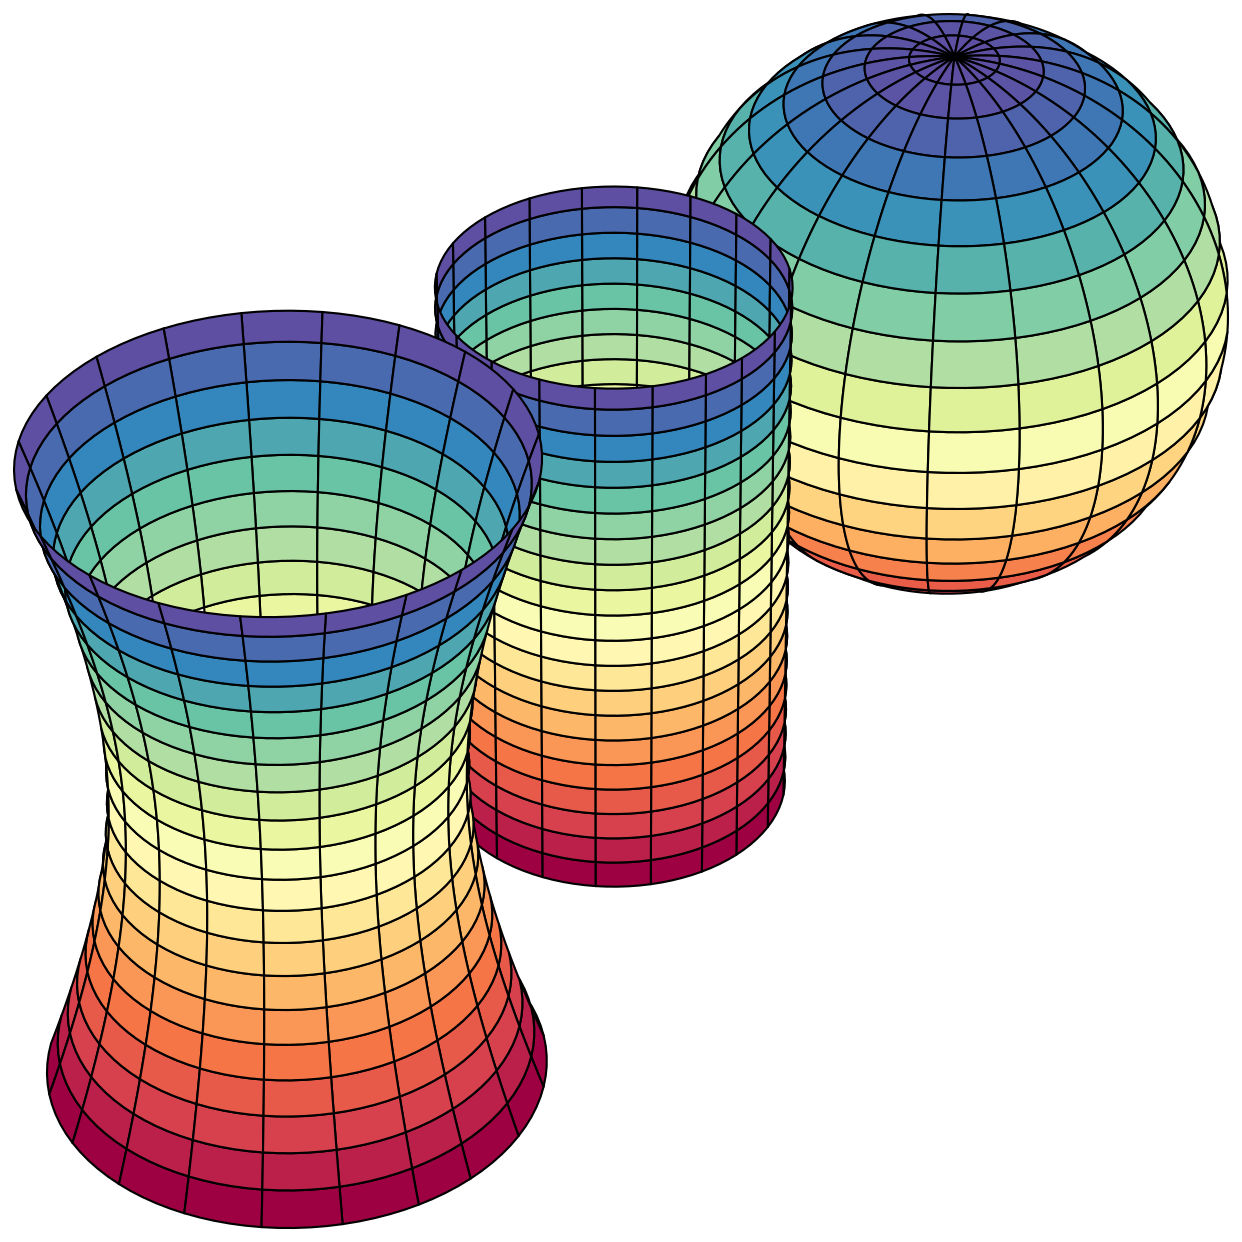
\includegraphics[height=2.7cm]{assets/colon-en/gaussian_curvature.png}\\[2pt]
      {\scriptsize $K\!<\!0$ 鞍面 \textperiodcentered\ $K\!=\!0$ 柱面 \textperiodcentered\ $K\!>\!0$ 球面。\\
       图：Nicoguaro，\href{https://commons.wikimedia.org/wiki/File:Gaussian_curvature.svg}{Wikimedia Commons}，CC0。}
    \end{column}
  \end{columns}
  \TLtakeaway{乘积 $\kappa_1\kappa_2$ 正是候选：柱面为 $0$（有一个因子为零），球面非零。这个乘积就是 Gauss 曲率。}
\end{frame}

% --- 2.2 Gauss curvature ----------------------------------------------------
\begin{frame}{Gauss 曲率 $K=\kappa_1\kappa_2$，算给你看}
  \[
    \boxed{\,K=\kappa_1\kappa_2\,}\qquad\Longrightarrow\qquad
    K_{\text{柱面}}=\tfrac1r\cdot 0=0,\qquad
    K_{\text{球面}}=\tfrac1R\cdot\tfrac1R=\tfrac{1}{R^2}.
  \]
  \begin{itemize}
    \item 柱面（$K=0$）正是那个能摊开的形状；球面（$K\neq0$）正是度量抹不平的那个。
    \item \textbf{猜想}：$K$ 就是障碍——只有 $K=0$ 处，曲面才能无畸变摊平。
  \end{itemize}
  但有个看似要命的麻烦：$\kappa_1,\kappa_2$ 描述曲面\emph{在空间里}怎么弯（外蕴），而只知道 $E,F,G$ 的「面内蚂蚁」似乎无从知道 $K$。下一页就是拯救这个猜想的奇迹。
  \TLtakeaway{$K$ 把「能摊平」（柱面 $K{=}0$）和「不能」（球面 $K{\neq}0$）分开。要把它做成定理，得让 $K$ 仅凭度量就能测出。}
\end{frame}

% --- 2.3 Theorema Egregium --------------------------------------------------
\begin{frame}{Gauss 的奇迹：$K$ 是内蕴的（绝妙定理）}
  \TLresultblock{绝妙定理（Gauss，1827）}{$K=\kappa_1\kappa_2$ 虽然\emph{由}曲面在空间里的弯曲来定义，却其实只用度量 $E,F,G$ 及其导数就能算出。所以 $K$ 是\TLterm{内蕴（intrinsic）}的：面内蚂蚁就能测出它。}
  \medskip
  我们要用的推论：\textbf{等距保持度量，因而保持 $K$}。
  \begin{itemize}
    \item 我们只用\emph{容易}的那一半：某处 $K\neq0$ $\Rightarrow$ 那里无法等距摊平。（逆命题「$K\equiv0\Rightarrow$ 局部平直」是 Minding 定理——引用即可，用不到。）
  \end{itemize}
  \TLinfoblock{完整证明（引用，不是糊弄）}{一般证明（Brioschi 公式）约两页：见 \href{https://en.wikipedia.org/wiki/Theorema_Egregium}{Theorema Egregium} 与 do~Carmo，\emph{Diff.\ Geometry of Curves \& Surfaces}，\S4-3。我们把 $K$ 的内蕴性当作已知；下一页\emph{完整}证明的是它推出的那个不可能性。}
\end{frame}

% --- 2.4 impossibility proven -----------------------------------------------
\begin{frame}{不可能性，证给你看}
  \begin{columns}[T]
    \begin{column}{0.58\textwidth}
      假设存在一个等距摊平 $\phi:S\to\text{平面}$。那么：
      \begin{enumerate}
        \item $\phi$ 是等距 $\Rightarrow$ 保持度量 $\Rightarrow$（绝妙定理）在对应点保持 $K$。
        \item 平面处处 $K=0$。
        \item 于是 $S$ 上处处 $K_S=0$。
        \item 但结肠的皱襞把它弯成两个方向，所以在一片正面积上 $K_S\neq0$。
      \end{enumerate}
      第 3、4 步矛盾。故 $\phi$ 不存在。
    \end{column}
    \begin{column}{0.42\textwidth}
      \TLresultblock{不存在无畸变的摊平}{结肠上某处 $K\neq0$ $\;\Longrightarrow\;$ \textbf{不存在到平面的等距映射。}你保不住所有长度。到此为止。}
    \end{column}
  \end{columns}
  \TLtakeaway{这是一个干净的「不行」，也是后文的设计约束：我们必须舍弃点什么。Q3 问——舍弃\emph{什么}？}
\end{frame}

% =============================================================================
\TLsection{Q3 · 等距已死，为什么保角度？}

% --- 3.1 the choice (weakest-link fix) --------------------------------------
\begin{frame}{摊平能保住的三样东西——挑一个}
  一张到平面的映射可以试着保住\textbf{长度}、\textbf{角度}或\textbf{面积}。长度做不到（Q2）。角度和面积之间，哪个对医生有用？
  \begin{columns}[T]
    \begin{column}{0.54\textwidth}
      \TLinfoblock{保角度（共形）}{息肉是靠它\emph{圆圆的形状}被认出来的。保角的映射把圆送成圆，于是医生靠形状的判读在摊平后依然成立。}
    \end{column}
    \begin{column}{0.46\textwidth}
      \TLwarnblock{改保面积呢？}{保面积的映射会把形状剪切——圆息肉被压成椭圆，恰恰毁掉医生依赖的那条线索。而面积误差只是一个全局因子，可以上色、可以标注。}
    \end{column}
  \end{columns}
  \medskip
  所以我们保\textbf{角度}，在\textbf{面积}上付账。保角度的映射叫作\TLterm{共形（conformal）}。
  \TLtakeaway{「让形状仍然可读」这个临床理由，才是逼我们选保角而非保面积的原因——不是随手的数学口味。}
\end{frame}

% --- 3.2 conformal defined + shown ------------------------------------------
\begin{frame}{共形 $=$ 把度量乘一个正因子}
  \TLterm{共形映射}：拉回的度量等于原度量乘一个正的标量场，
  \[
    \phi^{*}g_{\text{平面}}=e^{2u}\,g,\qquad e^{2u}>0\ \text{即\TLterm{共形因子（conformal factor）}}.
  \]
  为什么它保角、却要付面积——三行验算。把 $g\mapsto e^{2u}g$：
  \[
    \cos\angle=\frac{\inner{a}{b}_{e^{2u}g}}{\nm{a}_{e^{2u}g}\,\nm{b}_{e^{2u}g}}
    =\frac{e^{2u}\inner{a}{b}_g}{e^{u}\nm{a}_g\cdot e^{u}\nm{b}_g}
    =\frac{\inner{a}{b}_g}{\nm{a}_g\nm{b}_g}\quad(\textbf{角度不变}),
  \]
  而面积元 $\dd A=\sqrt{\det g}\,\dd u\,\dd v$ 变成 $\sqrt{\det(e^{2u}g)}=e^{2u}\sqrt{\det g}$（\textbf{面积} $\times e^{2u}$）。
  \TLtakeaway{这一个因子 $e^{2u}$ 在角度的比值里抵消，却把面积乘上去。角度免费，面积是全部账单——正是我们想要的交易。}
\end{frame}

% --- 3.3 circle stays circle + concrete number ------------------------------
\begin{frame}{一幅图加一个数：圆仍是圆}
  \begin{columns}[T]
    \begin{column}{0.56\textwidth}
      因为各个方向\emph{等比例}缩放，映射的 Jacobian 是 $e^{u}\times(\text{旋转})$。所以无穷小圆映成无穷小\emph{圆}——只改大小，绝不剪切成椭圆。
      \medskip
      一个具体因子：半径 $1$ 的球面的球极投影到平面是共形的，
      \[
        e^{2u}(\rho)=\frac{4}{(1+\rho^2)^2},
      \]
      其中 $\rho$ 是到中心的平面距离。$\rho=0$ 处面积放大 $4$ 倍，$\rho=1$ 处为 $1$——形状处处保圆，只有大小在呼吸。
    \end{column}
    \begin{column}{0.44\textwidth}
      \centering
      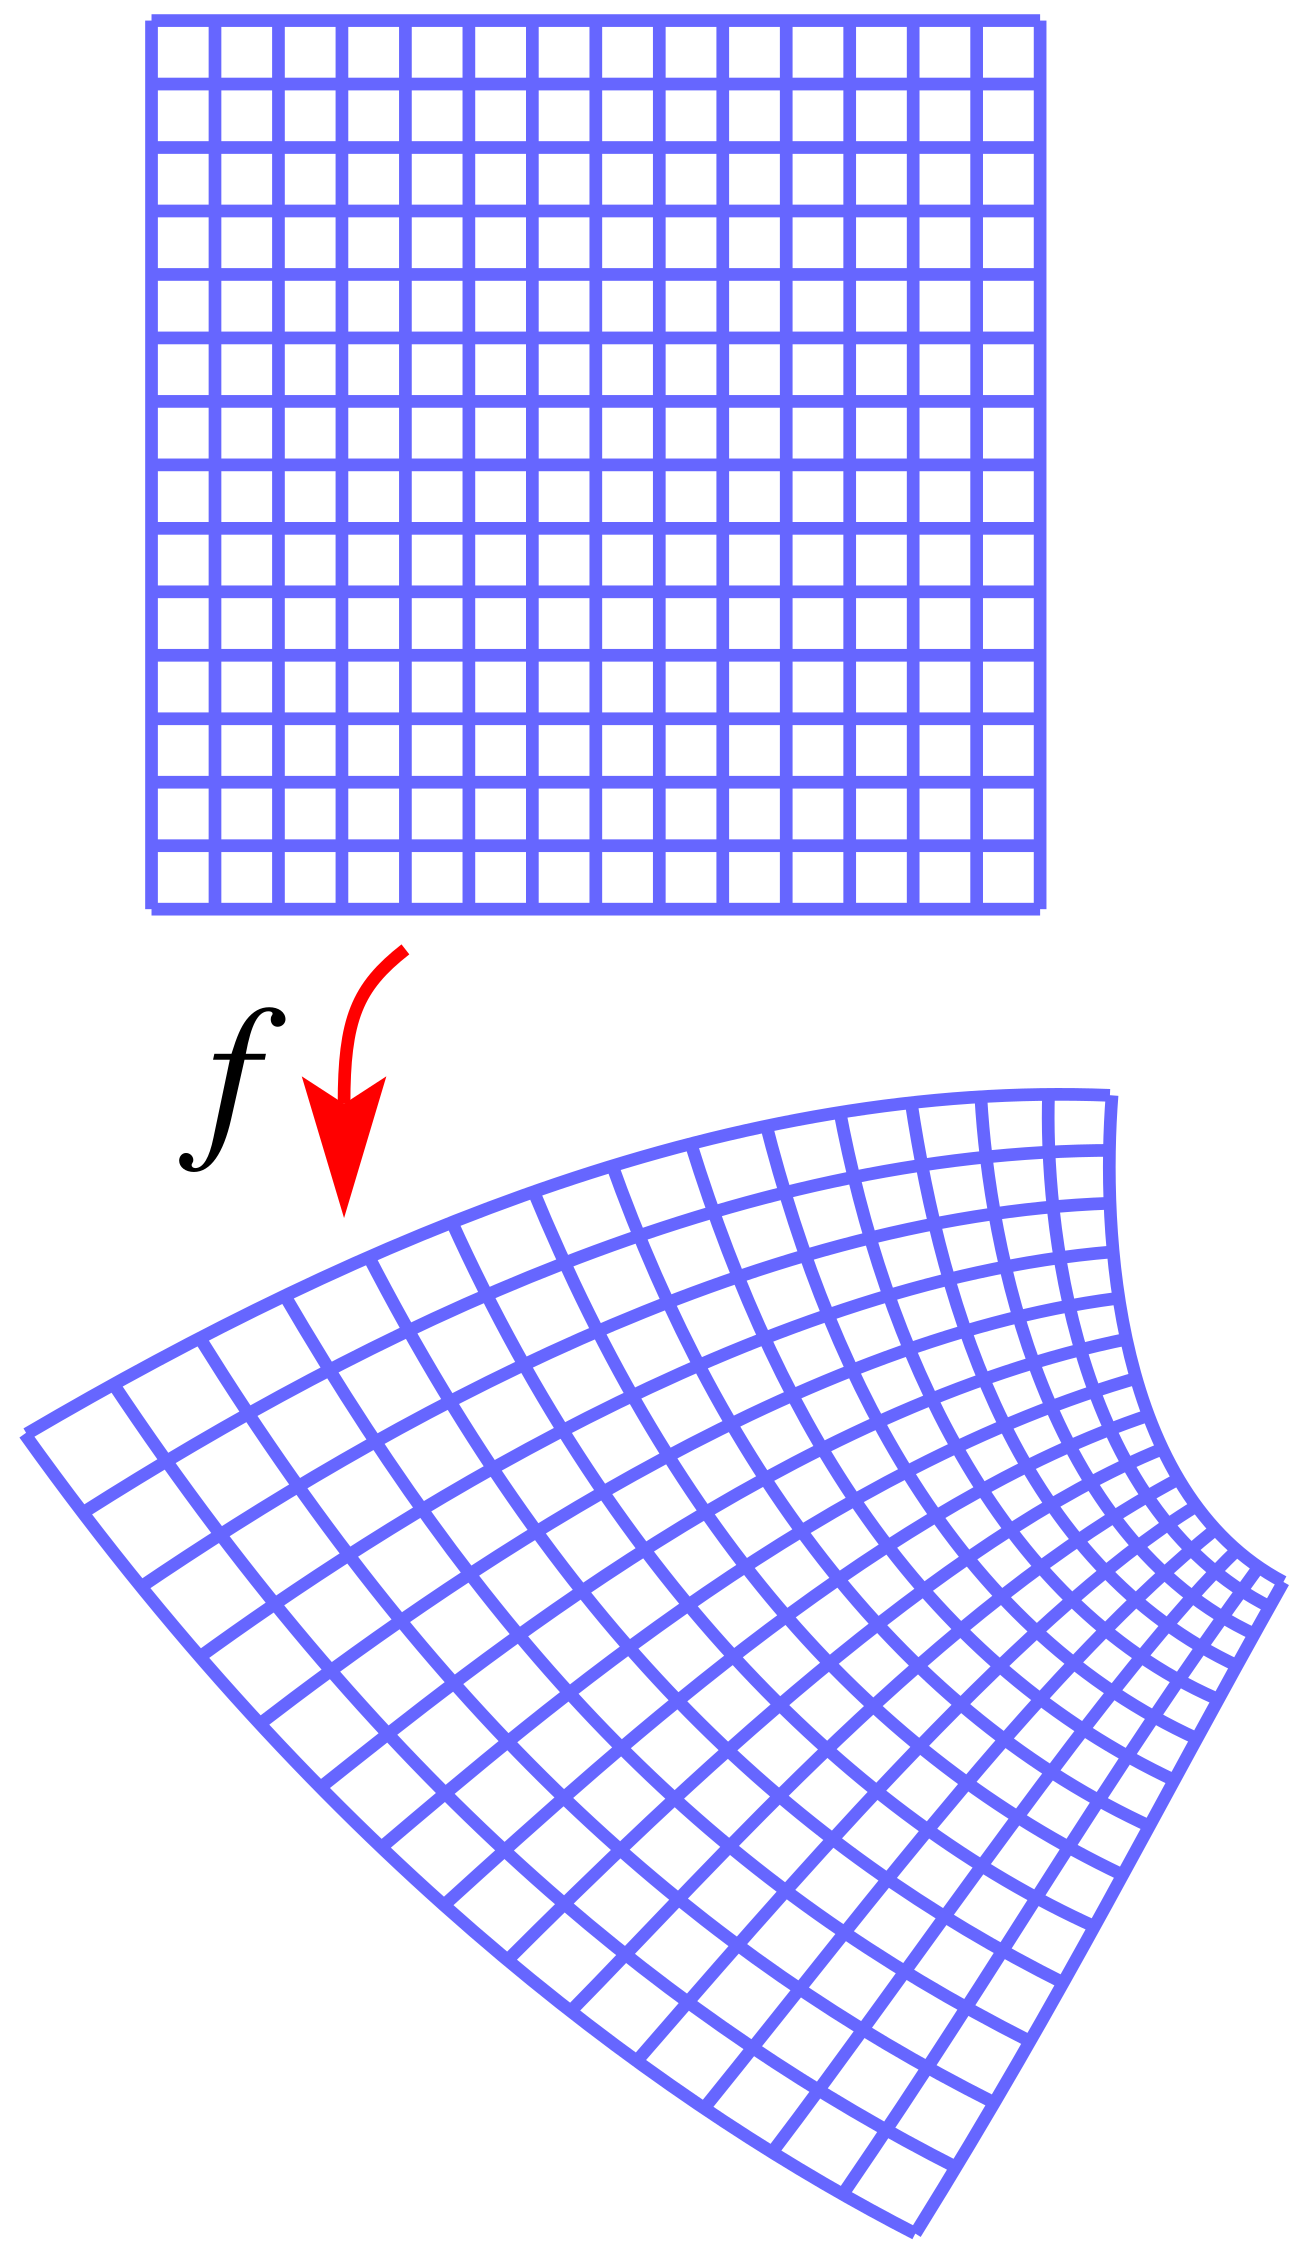
\includegraphics[height=4.0cm]{assets/colon-en/conformal_map.png}\\[2pt]
      {\scriptsize 共形映射 $f$：网格弯了，但每个交叉处仍是直角。\\
       图：Oleg Alexandrov，\href{https://commons.wikimedia.org/wiki/File:Conformal_map.svg}{Wikimedia Commons}，公有领域。}
    \end{column}
  \end{columns}
  \TLtakeaway{「保角」就是字面意义上的「让圆的东西仍然圆」。代价 $e^{2u}$ 现在是个你能从真实映射上读出来的数。}
\end{frame}

% --- 3.4 honesty + bridge ---------------------------------------------------
\begin{frame}{共形的摊平当真存在吗？（一句诚实的提醒）}
  \begin{columns}[T]
    \begin{column}{0.58\textwidth}
      对\emph{光滑}的结肠，「存在到平面的共形映射」这句话本身是一条深定理——\href{https://en.wikipedia.org/wiki/Uniformization_theorem}{单值化定理}。我们\textbf{不}证明它，也诚实地标出来：在光滑图景里，存在性我们暂且采信。
      \begin{itemize}
        \item 好消息：我们手里从来没有一个光滑结肠。
        \item 我们手里是一张\textbf{三角网格}。在网格上，摊平就是一个线性系统的解——\emph{存在性由线性代数白送}，不需要深定理。
      \end{itemize}
    \end{column}
    \begin{column}{0.42\textwidth}
      \TLinfoblock{Q4 交付的东西（先把范围说清）}{我们做的是带固定边界的离散\emph{调和}映射：极限意义下保角，$\approx$ 共形。把它做到\emph{精确}共形是后续讲义。我们对此说得很清楚，不夸大。}
    \end{column}
  \end{columns}
  \TLtakeaway{离散世界绕开了那条难的存在性定理：摊平之所以存在，是因为一个正定线性系统总有唯一解。现在就把它做出来。}
\end{frame}

% =============================================================================
\TLsection{Q4 · 在网格上算——不需要单值化}

% --- 4.1 discrete plan + win ------------------------------------------------
\begin{frame}{方案，以及它为什么不可能没有解}
  一次结肠扫描化成一张\TLterm{三角网格}：顶点、边、三角形。函数取\TLterm{分片线性（piecewise-linear）}——每个顶点一个值 $f_i$，三角形内部线性。
  \begin{columns}[T]
    \begin{column}{0.6\textwidth}
      \begin{itemize}
        \item 摊平的每个平面坐标，都求成一个\textbf{调和}函数：边界钉住后，最光滑、拉伸最小的场。
        \item 「调和」会化成一个\textbf{线性系统} $\Lmat x=b$，边界一旦固定，矩阵就是对称正定。
        \item 正定系统\emph{恰有一个}解。所以摊平总存在且唯一——\textbf{无需任何单值化定理}。
      \end{itemize}
    \end{column}
    \begin{column}{0.4\textwidth}
      \centering
      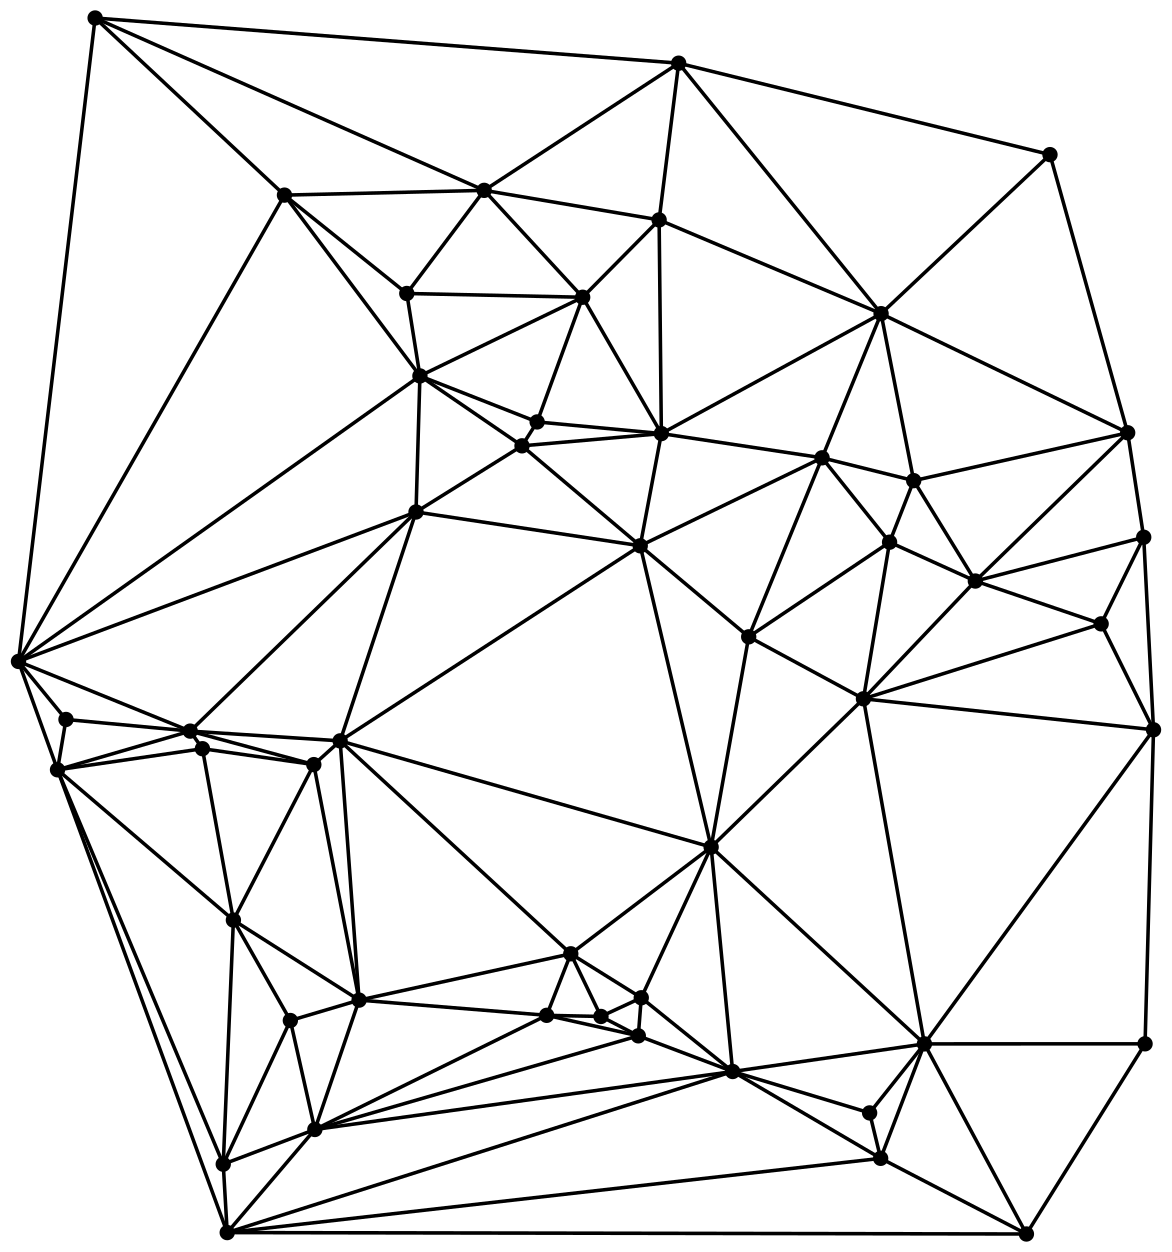
\includegraphics[height=3.3cm]{assets/colon-en/delaunay_mesh.png}\\[2pt]
      {\scriptsize 一张三角网格（Delaunay）。\\
       图：Inductiveload，\href{https://commons.wikimedia.org/wiki/File:Delaunay_Triangulation_(50_Points).svg}{Wikimedia Commons}，公有领域。}
    \end{column}
  \end{columns}
  \TLtakeaway{整个方法归结为：装出一个矩阵 $\Lmat$，再解 $\Lmat x=b$。Q4 余下的事就是：$\Lmat$ 从哪来，以及在一张小网格上手算它。}
\end{frame}

% --- 4.2 dirichlet energy bridge --------------------------------------------
\begin{frame}{拉伸最小 $=$ Dirichlet 能量 $=$ 调和}
  「保角、不乱起伏」由「拉伸总量最小」来刻画——即 \TLterm{Dirichlet 能量}：
  \[
    E_D(f)=\half\int_S \nm{\grad f}^2\,\dd A .
  \]
  \begin{itemize}
    \item 它（在边界固定下）的极小元是\TLterm{调和}函数：$\Lap f=0$。这是 Q2 曲率方程里那个 Laplace 算子的离散回声——算子重新登场，这次来干活。
    \item 二维里，\emph{共形}映射的坐标是调和的；精确的联系是 \href{https://en.wikipedia.org/wiki/Cauchy-Riemann_equations}{Cauchy--Riemann} 条件，它需要复分析——这里暂且采信，留到后续讲义证明。所以在固定边界下极小化 $E_D$ 给出调和坐标：\emph{在共形极限意义下}保角，而非对任意边界都保角。
  \end{itemize}
  \TLtakeaway{我们要的不是映射的公式，而是那个「拉伸最小」的场。接下两页把网格上的 $E_D$ 变成矩阵，cotangent 会自己冒出来。}
\end{frame}

% --- 4.3 PL gradient --------------------------------------------------------
\begin{frame}{一个三角形：帽函数的梯度}
  \begin{columns}[T]
    \begin{column}{0.56\textwidth}
      在三角形 $T=(i,j,k)$ 上，\textbf{帽函数} $\varphi_i$ 线性，在 $i$ 处为 $1$、在对边 $jk$ 上为 $0$。
      \begin{itemize}
        \item 它的梯度 $\grad\varphi_i$ 在 $T$ 上\emph{是常向量}，垂直于对边 $jk$，长度为 $1/h_i$，其中 $h_i$ 是 $i$ 到 $jk$ 的高。
        \item 于是分片线性的 $f=\sum_i f_i\varphi_i$ 在每个三角形上梯度为常向量。
      \end{itemize}
      常梯度让能量积分变得平凡：它就是（面积）$\times$（点积）。
    \end{column}
    \begin{column}{0.44\textwidth}
      \centering
      \begin{tikzpicture}[scale=1.1,every node/.style={font=\scriptsize}]
        \coordinate (i) at (0,0); \coordinate (j) at (2.0,0.1); \coordinate (k) at (0.7,1.5);
        \draw[fill=TLprimaryTint] (i)--(j)--(k)--cycle;
        \foreach \p/\l in {i/i,j/j,k/k}{\fill (\p) circle (1.2pt); \node at ($(\p)+(0,0.2)$) {$\l$};}
        \coordinate (foot) at ($(j)!(i)!(k)$);   % foot of perpendicular from i onto edge jk
        \draw[->,TLaccent,very thick] (foot)--(i);
        \node[TLaccent,above left] at ($(foot)!0.5!(i)$) {$\grad\varphi_i$};
        \node[TLneg,below right] at ($(foot)!0.5!(i)$) {$h_i$};
        \node at (1.0,-0.45) {$\grad\varphi_i\perp jk$，指向 $i$};
      \end{tikzpicture}
    \end{column}
  \end{columns}
  \TLtakeaway{唯一需要的几何事实：$\grad\varphi_i\perp jk$，长度 $1/h_i$。下一页 cotangent 就从它落出来。}
\end{frame}

% --- 4.4 cotangent appears --------------------------------------------------
\begin{frame}{cotangent 冒出来（值得做一次的那一步）}
  能量要用到 $\displaystyle\int_T\grad\varphi_i\cdot\grad\varphi_j\,\dd A$。两个梯度都是常向量，所以它等于 $\text{面积}\cdot(\grad\varphi_i\cdot\grad\varphi_j)$。记 $a=\nm{jk},\,b=\nm{ik}$，$\theta_k$ 为 $k$ 处的角。
  \[
    \grad\varphi_i\perp jk,\ \grad\varphi_j\perp ik\ \Rightarrow\
    \grad\varphi_i\cdot\grad\varphi_j=\frac{\cos(\pi-\theta_k)}{h_i h_j}=-\frac{ab\cos\theta_k}{4\,\text{面积}^2}
    \quad\Big(h_i=\tfrac{2\text{面积}}{a},\,h_j=\tfrac{2\text{面积}}{b}\Big).
  \]
  乘上面积，再用 $\text{面积}=\half ab\sin\theta_k$：
  \[
    \int_T\grad\varphi_i\cdot\grad\varphi_j\,\dd A=-\frac{ab\cos\theta_k}{4\,\text{面积}}
    =-\frac{ab\cos\theta_k}{2ab\sin\theta_k}=\boxed{-\half\cot\theta_k}.
  \]
  \TLtakeaway{cotangent 不是约定，而是 $\cos\theta_k/\sin\theta_k$：$\cos$ 来自两个梯度之间的夹角，$\sin$ 来自三角形的面积。这一步你刚刚把方法的核心亲手重推了一遍。}
\end{frame}

% --- 4.5 assemble + Laplacian + signs ---------------------------------------
\begin{frame}{装配：cotangent Laplacian}
  一条内部边 $(i,j)$ 被两个三角形共享，记这条边\emph{所对}的两个角为 $\alpha_{ij},\beta_{ij}$。把两个三角形相加，能量变成
  \[
    E_D(f)=\half\sum_{\text{边 }(i,j)} w_{ij}\,(f_i-f_j)^2,\qquad
    \boxed{\,w_{ij}=\half(\cot\alpha_{ij}+\cot\beta_{ij})\,}.
  \]
  \begin{columns}[T]
    \begin{column}{0.6\textwidth}
      极小化（在内部顶点令 $\partial E_D/\partial f_i=0$）给出 \TLterm{cotangent Laplacian}：
      \[
        (\Lmat f)_i=\sum_{j\sim i} w_{ij}(f_i-f_j)=0 .
      \]
      矩阵元 $L_{ii}=\sum_j w_{ij},\ L_{ij}=-w_{ij}$：对称、半正定，\textbf{边界一旦固定即正定}。
    \end{column}
    \begin{column}{0.4\textwidth}
      \centering
      \begin{tikzpicture}[scale=0.66,every node/.style={font=\scriptsize}]
        \coordinate (i) at (0,0); \coordinate (j) at (2.1,0.15);
        \coordinate (k) at (1.0,1.4); \coordinate (l) at (1.05,-1.3);
        \draw[fill=TLprimaryTint] (i)--(k)--(j)--cycle;
        \draw[fill=TLprimaryTint] (i)--(l)--(j)--cycle;
        \draw[very thick,TLaccent] (i)--(j);
        \foreach \p/\l in {i/i,j/j,k/k,l/l}{\fill (\p) circle (1.2pt); \node[above] at (\p) {$\l$};}
        \node[TLprimary] at (1.0,1.0) {$\alpha_{ij}$};
        \node[TLprimary] at (1.05,-0.85) {$\beta_{ij}$};
      \end{tikzpicture}\\[1pt]
      {\scriptsize 角不太钝时 $w_{ij}>0$（Delaunay）。}
    \end{column}
  \end{columns}
  \TLtakeaway{「求调和摊平」现在就是字面上的「解 $\Lmat x=b$」。一条装配规则，每个坐标一次稀疏正定求解。}
\end{frame}

% --- 4.6 boundary conditions ------------------------------------------------
\begin{frame}{钉住边界，解出内部}
  光有 $\Lmat f=0$ 解不唯一（常数也是调和的）。我们靠\textbf{固定边界}——剪开后结肠的那圈边沿——把解定死：
  \begin{itemize}
    \item 选定边界这个圈落到平面的什么位置（一个圆或一个方框）。
    \item 把这些边界顶点钉住，只对\emph{内部}顶点解 $\Lmat x=b$，其中 $b$ 收集被钉住的边界项。
    \item 边界固定后，$\Lmat$（限制到内部顶点）正定 $\Rightarrow$ 内部布局唯一。
  \end{itemize}
  这正是 Q3 那个诚实的范围：带选定边界的\emph{调和}映射——极限意义下保角，$\approx$ 共形。边界的选取是唯一的自由决定。
  \TLtakeaway{边界固定 $\Rightarrow$ 正定 $\Rightarrow$ 摊平唯一。不靠存在性定理，只靠线性代数。该上手算了。}
\end{frame}

% --- 4.7 worked example -----------------------------------------------------
\begin{frame}{手算：一个内部顶点}
  \begin{columns}[T]
    \begin{column}{0.5\textwidth}
      取一个正六边形扇：六个边界顶点、一个内部顶点 $c$，六个等边三角形。每个角都是 $60^\circ$，于是每条辐边的权都相等：
      \[
        w_{ci}=\half(\cot 60^\circ+\cot 60^\circ)=\tfrac{1}{\sqrt3}.
      \]
      权相等，内部方程就塌缩成一个平均：
      \[
        \sum_{i=1}^{6} w_{ci}(x_c-x_i)=0\ \Rightarrow\ x_c=\tfrac{1}{6}\textstyle\sum_i x_i .
      \]
    \end{column}
    \begin{column}{0.5\textwidth}
      把边界钉到正六边形 $p_i=(\cos 60^\circ i,\ \sin 60^\circ i)$。它们的平均是 $(0,0)$，所以 $x_c=(0,0)$，即形心。改钉一个\emph{不规则}六边形，$x_c$ 仍是那六个被钉点的普通平均——一行算术。
      \smallskip
      你刚刚把整个算法走了一个缩微版：装配 $\Lmat$（这里是 $1\times1$ 系统），加边界条件，求解。
    \end{column}
  \end{columns}
  \TLtakeaway{调和 $=$ 每个自由顶点是其邻居的 cotangent 加权平均。角相等给普通平均；角不等，给真正的加权平均。}
\end{frame}

% --- 4.8 algorithm summary --------------------------------------------------
\begin{frame}{算法，五行讲完}
  \begin{enumerate}
    \item \textbf{剪开}结肠这根管子，沿一条曲线剪；现在它是一个带边界的圆盘。
    \item \textbf{剖分}成三角形；读出每个三角形的角。
    \item \textbf{装配} $\Lmat$，权 $w_{ij}=\half(\cot\alpha_{ij}+\cot\beta_{ij})$。
    \item \textbf{钉住}边界圈到一个圆/方框；对内部\textbf{解} $\Lmat x=b$（两个坐标，两次正定求解）。
    \item \textbf{铺平}：把网格放到解出的位置——摊平后的结肠。
  \end{enumerate}
  \TLwarnblock{诚实的范围}{这是离散\emph{调和}参数化。它在极限意义下保角（$\approx$ 共形），并非精确共形。做到精确（极小化 Cauchy--Riemann 残差 / LSCM）是后续讲义。}
  \TLtakeaway{五步，全是线性代数。唯一要拿主意的是边界形状。接下来：它守住承诺了吗，代价又是多少？}
\end{frame}

% =============================================================================
\TLsection{Q5 · 做出来了吗？代价是多少？}

% --- 5.1 angle check --------------------------------------------------------
\begin{frame}{承诺：角度（量出来，不是假设）}
  在摊平后的网格上验承诺：对每个三角形，比较映射前后的三个角。
  \begin{itemize}
    \item 对钉到正六边形的等边扇，映射是一个相似变换——每个角\emph{精确}保持，角度误差 $=0$。
    \item 对一般网格，离散调和映射只\emph{近似}保角：误差小但非零。（这个缺口，正是后续讲义那个精确共形方法要消去的。）
  \end{itemize}
  所以我们把角度误差报成一个\emph{量出来的残差}——接近零，但诚实地说一般并非恰好为零。
  \TLtakeaway{讲义不声称「角度误差 $=0$」，只声称「小且可测」——并明确告诉你哪个后续方法把它压到零。}
\end{frame}

% --- 5.2 area price ---------------------------------------------------------
\begin{frame}{代价：面积（一个真实的数）}
  面积是我们在 Q3 答应付的账。直接量它：对每个三角形，面积比
  \[
    \text{(面积畸变)}_T=\frac{\text{面积}\big(\phi(T)\big)}{\text{面积}(T)} .
  \]
  \begin{itemize}
    \item 这个逐三角形的比，是 Q3 共形因子 $e^{2u}$ 的离散采样版——现在是每个三角形上的一个具体数，而非符号。
    \item 原结肠弯得最厉害（深皱襞、$|K|$ 大）的地方，这个比偏离 $1$ 最多：那些片被明显放大或压缩。
  \end{itemize}
  \TLtakeaway{角度几乎免费拿到；面积没有。这些比值的直方图\emph{就是}那张账单——而它最大的地方，恰恰是结肠最弯的地方。}
\end{frame}

% --- 5.3 close the loop -----------------------------------------------------
\begin{frame}{闭合环：账单就是你抹不掉的曲率}
  面积畸变不是运气不好——它由 Q2 强制。离散 Gauss--Bonnet 恒等式把它量化：
  \[
    \sum_{\text{内部 } i}\Big(2\pi-\!\!\sum_{i\text{ 处的角}}\!\!\theta\Big)=2\pi\chi(S)\quad\text{（总角亏}=\text{总曲率）} .
  \]
  \begin{itemize}
    \item 平直布局在内部顶点处角亏为\emph{零}。结肠的角亏非零（它的曲率，来自 Q2）。
    \item 这个差消不掉——只能\emph{挪}进我们留的那一条通道：面积。所以 Q2 里非零的曲率\emph{保证}了 Q5 里非零的面积畸变。
  \end{itemize}
  \TLtakeaway{你在 Q5 量到的那个数，早在 Q2 证明 $K\neq0$ 时就注定了。讲义自己闭合了环：代价等于你从一开始就不被允许抹掉的曲率。}
\end{frame}

% --- 5.4 clinical reading ---------------------------------------------------
\begin{frame}{读摊平后的结肠（一份诚实的使用说明）}
  \begin{columns}[T]
    \begin{column}{0.5\textwidth}
      \TLinfoblock{可信}{局部\emph{形状}。息肉仍然圆，皱襞保住其角度结构。靠形状的检测在摊平图上有效。}
    \end{column}
    \begin{column}{0.5\textwidth}
      \TLwarnblock{别信}{绝对\emph{大小}，尤其在面积比远离 $1$ 的深皱襞附近。读尺寸要对照面积畸变图，别照字面看。}
    \end{column}
  \end{columns}
  \medskip
  这就是全部的交易，说穿了：舍弃长度（被迫），保住角度（为形状而选），在面积上付账（量得出，且被曲率从下方限制）。
  \TLtakeaway{好的摊平不是无畸变，而是它那唯一的畸变\emph{已知、可定位、可解释}。这正是我们造出来的东西。}
\end{frame}

% =============================================================================
\TLsection{做了什么 · 接下来 · 符号表 · 习题 · 参考文献}

% --- synthesis / next decks -------------------------------------------------
\begin{frame}{我们做了什么，以及后续讲义}
  \begin{columns}[T]
    \begin{column}{0.56\textwidth}
      \textbf{这一讲，从头到尾：}
      \begin{itemize}
        \item 为什么不存在无畸变摊平（绝妙定理，证明了不可能性）。
        \item 为什么保角度（临床），以及代价是什么（面积 $=e^{2u}$）。
        \item 一个方法，完整搭起并手算：cotangent Laplacian、调和映射、固定边界。
      \end{itemize}
    \end{column}
    \begin{column}{0.44\textwidth}
      \textbf{后续讲义（同样深度搭建）：}
      \begin{itemize}
        \item \emph{精确}共形：极小化 Cauchy--Riemann 残差（LSCM）。
        \item 整体结构：全纯 1-形式 / Hodge 理论。
        \item 可编程目标曲率：Ricci 流。
      \end{itemize}
    \end{column}
  \end{columns}
  \TLtakeaway{一个问题、一个方法，彻底拿下——这是整个系列的模板。后面每一讲都拆掉本讲一条诚实的局限。}
\end{frame}

% --- notation ---------------------------------------------------------------
\begin{frame}{符号表 (Notation)（只列我们用过的）}
  \begin{columns}[T]
    \begin{column}{0.5\textwidth}
      \begin{tabular}{@{}ll@{}}
        $\xb(u,v)$ & 曲面（到 $\R^3$ 的映射）\\
        $\xb_u,\xb_v$ & 切向量（尺子）\\
        $E,F,G$ & 第一基本形式（度量）\\
        $\kappa_1,\kappa_2$ & 主曲率\\
        $K=\kappa_1\kappa_2$ & Gauss 曲率\\
      \end{tabular}
    \end{column}
    \begin{column}{0.5\textwidth}
      \begin{tabular}{@{}ll@{}}
        $e^{2u}$ & 共形因子（面积的代价）\\
        $\varphi_i$ & 顶点 $i$ 的帽函数\\
        $\alpha_{ij},\beta_{ij}$ & 边 $(i,j)$ 所对的两角\\
        $w_{ij}$ & cotangent 权\\
        $\Lmat$ & cotangent Laplacian（$\Lmat x=b$）\\
      \end{tabular}
    \end{column}
  \end{columns}
  \TLtakeaway{十个符号，每个都在某个问题需要它的地方出场。若这十个你都能凭记忆定义，你就能重推整份讲义。}
\end{frame}

% --- exercises --------------------------------------------------------------
\begin{frame}{习题 (Exercises)（做完这些，你才真正拥有它）}
  \begin{enumerate}
    \item \textbf{度量}：算柱面 $\xb=(r\cos u,r\sin u,v)$ 的 $E,F,G$，并验证一次重新标度把它变成平面度量。
    \item \textbf{曲率}：由球面的主曲率，验证 $K=1/R^2$；用一行说明为什么柱面 $K=0$。
    \item \textbf{cotangent}：对一个 $45^\circ$--$45^\circ$--$90^\circ$ 三角形，算出每个角对应的权贡献 $-\half\cot\theta_k$。
    \item \textbf{求解}：取那个一内部顶点的扇，把边界钉成你自选的一个\emph{不规则}六边形，解出内部顶点（它就是加权平均——算出一个数）。
    \item \textbf{闭环}：用离散 Gauss--Bonnet 论证，$K\neq0$ 的结肠在任何平直布局后\emph{必然}出现非零的面积畸变。
  \end{enumerate}
\end{frame}

% --- references -------------------------------------------------------------
\begin{frame}{参考文献 (References) 与图片出处}
  \footnotesize
  \begin{thebibliography}{9}
    \setbeamertemplate{bibliography item}[text]
    \bibitem{docarmo} M.~do Carmo. \emph{Differential Geometry of Curves and Surfaces}. Prentice-Hall, 1976.（度量、曲率、绝妙定理 --- \S2--\S4）
    \bibitem{egregium} \href{https://en.wikipedia.org/wiki/Theorema_Egregium}{Theorema Egregium} 与 \href{https://en.wikipedia.org/wiki/Gaussian_curvature}{Gaussian curvature}（Wikipedia）--- 完整陈述与 Brioschi 证明。
    \bibitem{uniform} \href{https://en.wikipedia.org/wiki/Uniformization_theorem}{Uniformization theorem}（Wikipedia）--- 光滑共形存在性，引用未证。
    \bibitem{cotan} \href{https://en.wikipedia.org/wiki/Discrete_Laplace_operator}{Discrete Laplace operator}（Wikipedia）--- 网格上的 cotangent 权。
    \bibitem{hat} S.~Haker, S.~Angenent, A.~Tannenbaum, R.~Kikinis. \emph{Nondistorting flattening maps and the 3D visualization of colon CT images}. IEEE TMI, 19(7), 2000.（调和结肠展开）
  \end{thebibliography}
  \smallskip
  {\scriptsize 图片出处（均为开放授权，经 Wikimedia Commons）：Gauss 曲率示意 --- Nicoguaro，CC0；结肠解剖 --- Mikael Häggström，公有领域；共形映射 --- Oleg Alexandrov，公有领域；三角网格 --- Inductiveload，公有领域。其余插图均为原创（TikZ）。}
\end{frame}

\end{document}
